\documentclass[llpt]{beamer}
\usepackage{physics}
\usepackage{hyperref}
\usepackage[font=tiny]{caption}

\mode<presentation>
{
  \usetheme{Warsaw}  
  \usecolortheme{beaver} 
  \usefonttheme{default} 
  \setbeamertemplate{navigation symbols}{}
  \setbeamertemplate{caption}[numbered]
  
  \setbeamertemplate{footline}[frame number]
}

\usepackage[english]{babel}
\usepackage[utf8x]{inputenc}


\title{Matrix Product States for Machine Learning}
\author{Jue Xu\inst{1} \and John Martyn\inst{1} \and Qingyang Tan\inst{1} \and Sanket Doshi\inst{1}}
\institute{\inst{1} University of Maryland, College Park}
\date{December 2019}

  

\begin{document}
\begin{frame}
  \titlepage
\end{frame}


\section{Introduction}

\subsection{Motivation}
\begin{frame}
\frametitle{Outline}
\begin{itemize}
    \item A rapid-fire introduction to tensor networks
    \item Matrix product states and DMRG optimization 
    \item Applications of MPS to MNIST, Fashion MNIST and CIFAR
    \item Outlook
\end{itemize}
\end{frame}


\begin{frame}{Tensor Networks}
  \begin{itemize}
      \item When analyzing quantum systems, it is convenient to represent tensorial quantities via tensor networks
      \item For instance, the state of an n particle system takes the form:
      \begin{equation}
      \ket{\Psi} = \sum_{i_1, i_2, ... i_n} C_{i_1, i_2, ... i_n} \ket{\psi_{i_1}} \otimes \ket{\psi_{i_2}} \otimes ... \otimes \ket{\psi_{i_n}} \quad \Rightarrow
      \end{equation}
  \end{itemize}
  \qquad \qquad \qquad 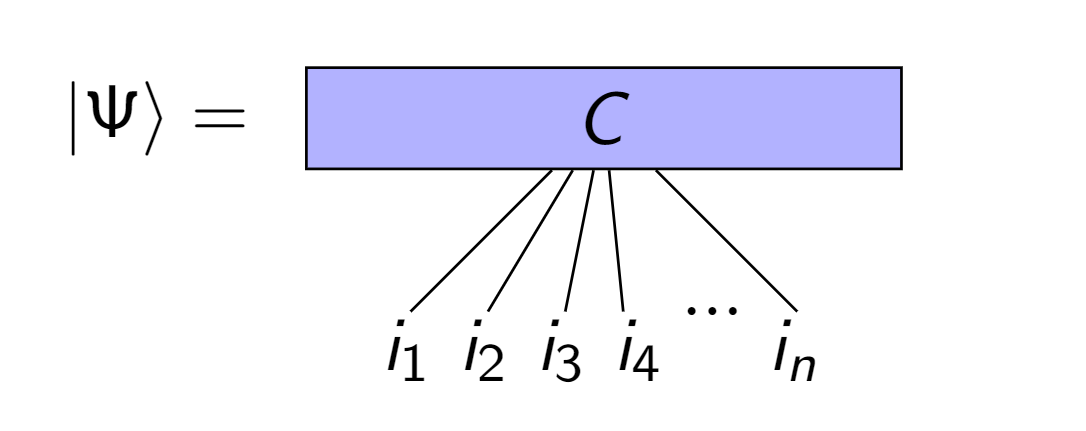
\includegraphics[width=.6\textwidth]{psi.PNG}
\end{frame}


\begin{frame}{Matrix Product States}
  \begin{itemize}
      \item A particularly useful tensor network is a matrix product state: $|\psi \rangle = \sum_{i_1, i_2, ..., i_N} \text{tr}(A^{(1)}_{i_1} A^{(2)}_{i_2} ... A^{(N)}_{i_N})\ |i_1 i_2... i_N \rangle $.
      \item Graphically [1], 
      \begin{figure}
      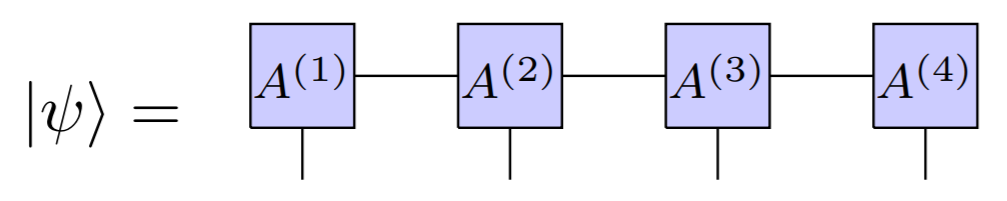
\includegraphics[width=.5\textwidth]{MPS.PNG}
      \end{figure}
      \begin{figure}
      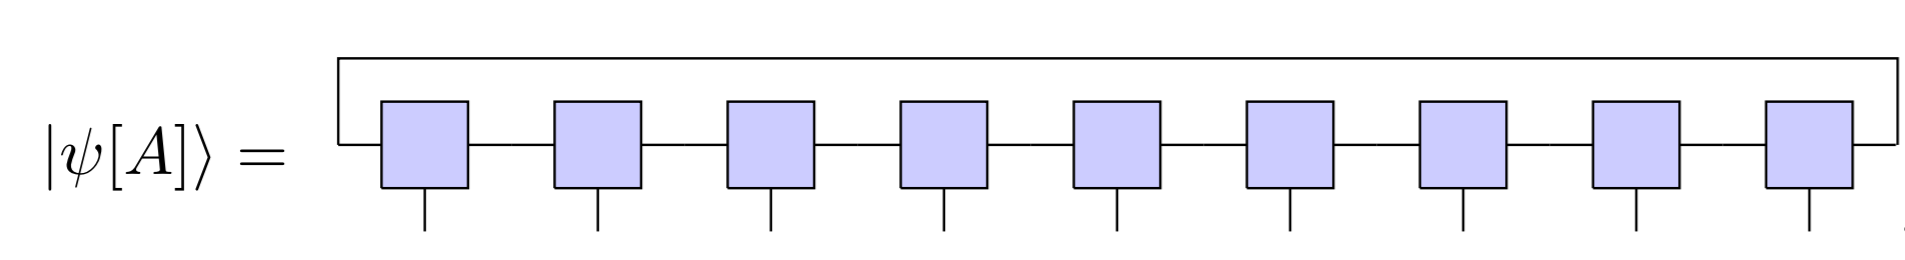
\includegraphics[width=.9\textwidth]{MPS_periodic.PNG}
      \end{figure} 
      \item The rank of $A^{(j)}_{i_j}$ is the bond dimension, $\chi$
      \item All quantum states admit an MPS representation for sufficiently large $\chi$ (might be infeasible in practice)
  \end{itemize}
\end{frame}


\begin{frame}{MPS for Machine Learning}
\begin{itemize}
    \item We can use MPS for classification: introduce label index $\ell$ [4].
    \item To determine the class of some data $|x \rangle$, take the overlap between the MPS and $ |x \rangle $. The class is the index for which this is largest [4]. 
\end{itemize}
\qquad \qquad
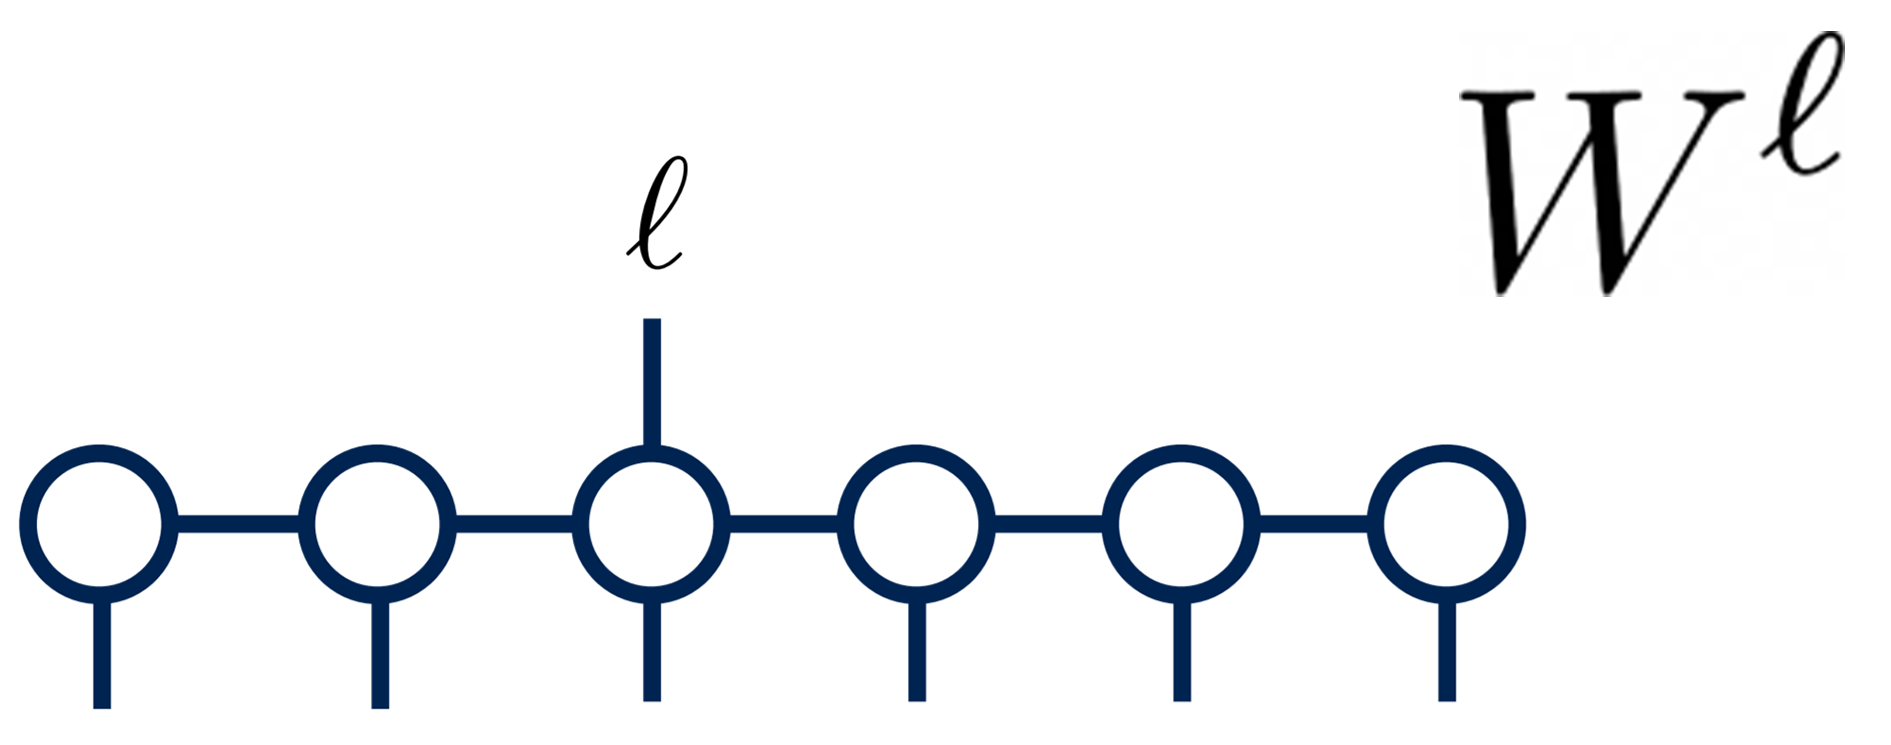
\includegraphics[width=.3\textwidth]{MPS_classification.PNG} \qquad
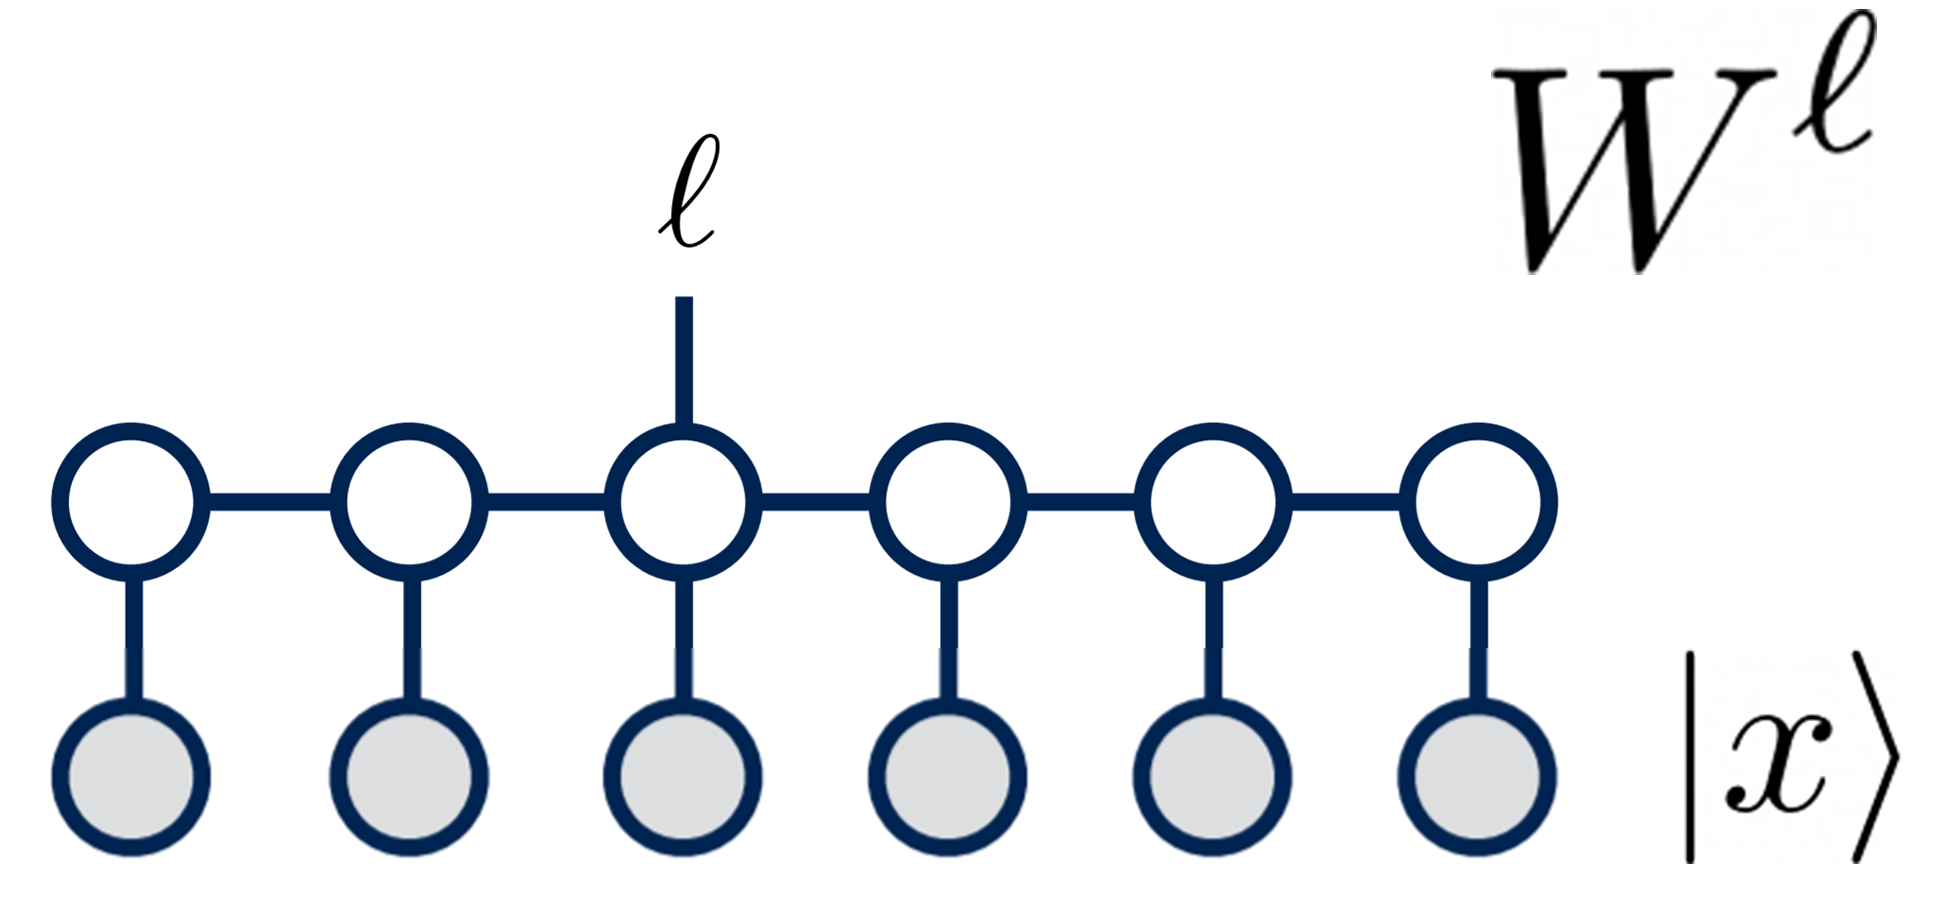
\includegraphics[width=.3\textwidth]{overlap.png}
\begin{itemize}
    \item Because we manipulate quantum states, this procedure can be deployed on a quantum computer to speed up training $\Rightarrow$ quantum machine learning
\end{itemize}
\end{frame}

\begingroup
\small
\begin{frame}{Sweeping algorithm of Stoudenmire and Schwab}
    \begin{itemize}
    \item Example: minimizing squared loss
    \begin{equation}
        C = \dfrac{1}{2}\sum_{n=1}^{N_T}\sum_{\ell}(W^{\ell}.\Phi(x_n)-\delta^{\ell}_{L_n})^2
    \end{equation}
    with an MPS ansatz\begin{equation}
        W^{\ell}_{s_1s_2\ldots s_N} = \sum_{\{\alpha\}}A^{\alpha_1}_{s_1}A^{\alpha_1\alpha_2}_{s_2}\ldots A^{\ell;\alpha_j\alpha_{j+1}}\ldots A^{\alpha_N-1}_{s_N}
    \end{equation}
     \begin{figure}
     \begin{subfigure}
   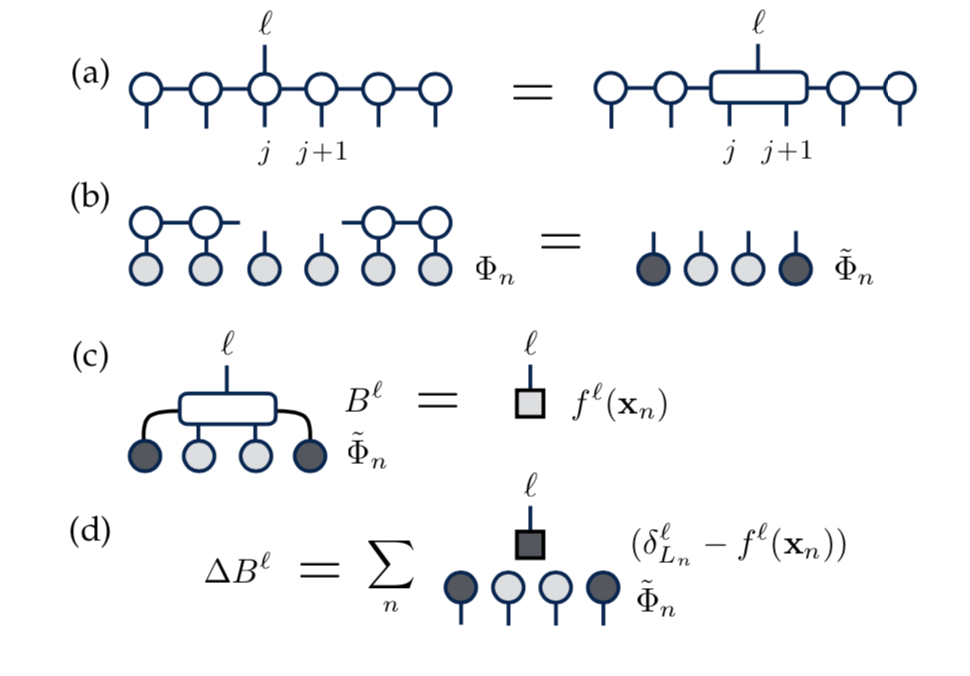
\includegraphics[width=0.42\textwidth]{opt_img1.png}
   \end{subfigure}
   \hfill
   \begin{subfigure}
   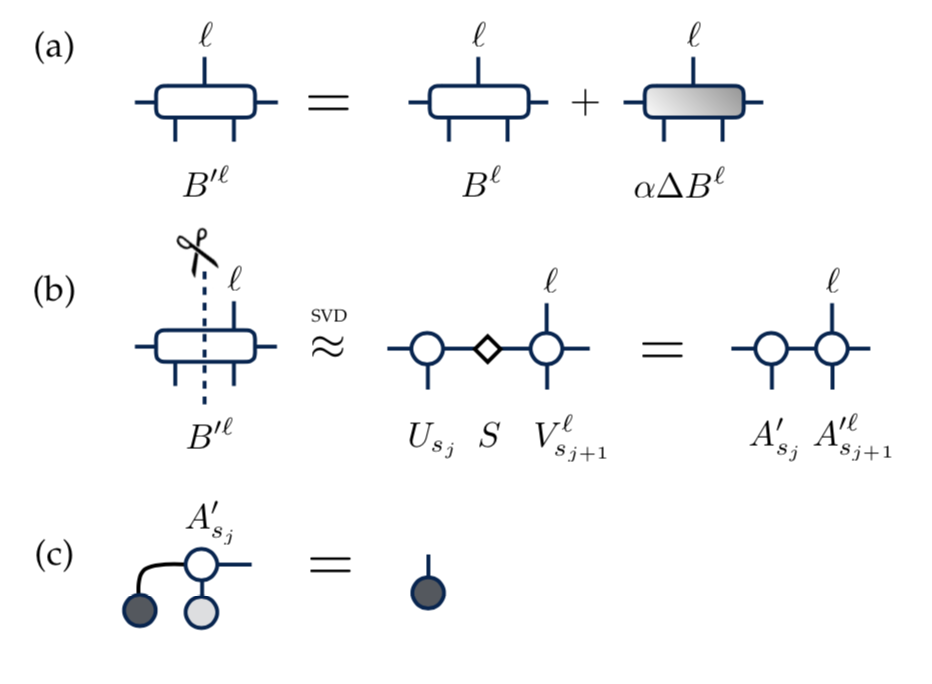
\includegraphics[width=0.42\textwidth]{opt_img2.png}
    \end{subfigure}
    \caption{Images taken from [4]}
    \end{figure}
   \end{itemize}
\end{frame}
\endgroup


\begin{frame}{Goals}
\begin{itemize}
    \item We seek to expand on previous studies and benchmark MPS for classification problems.
    \item We study the MNIST, FashionMNIST, and CIFAR data sets.
    \item Using TorchMPS, we analyze the accuracy for various MPS properties: bond dimension, L2 Regularization.
    \item We deploy the training algorithm on GPU.
\end{itemize}
\end{frame}

\begin{frame}{Results - Bond Dimension}
    \begin{itemize}
        \item We study MNIST for different bond dimensions (no regularization, 2000 train samples, 100 test)
        \item Higher bond dimension correlates to higher accuracy, as expected
    \end{itemize}
    \qquad  \qquad \qquad
    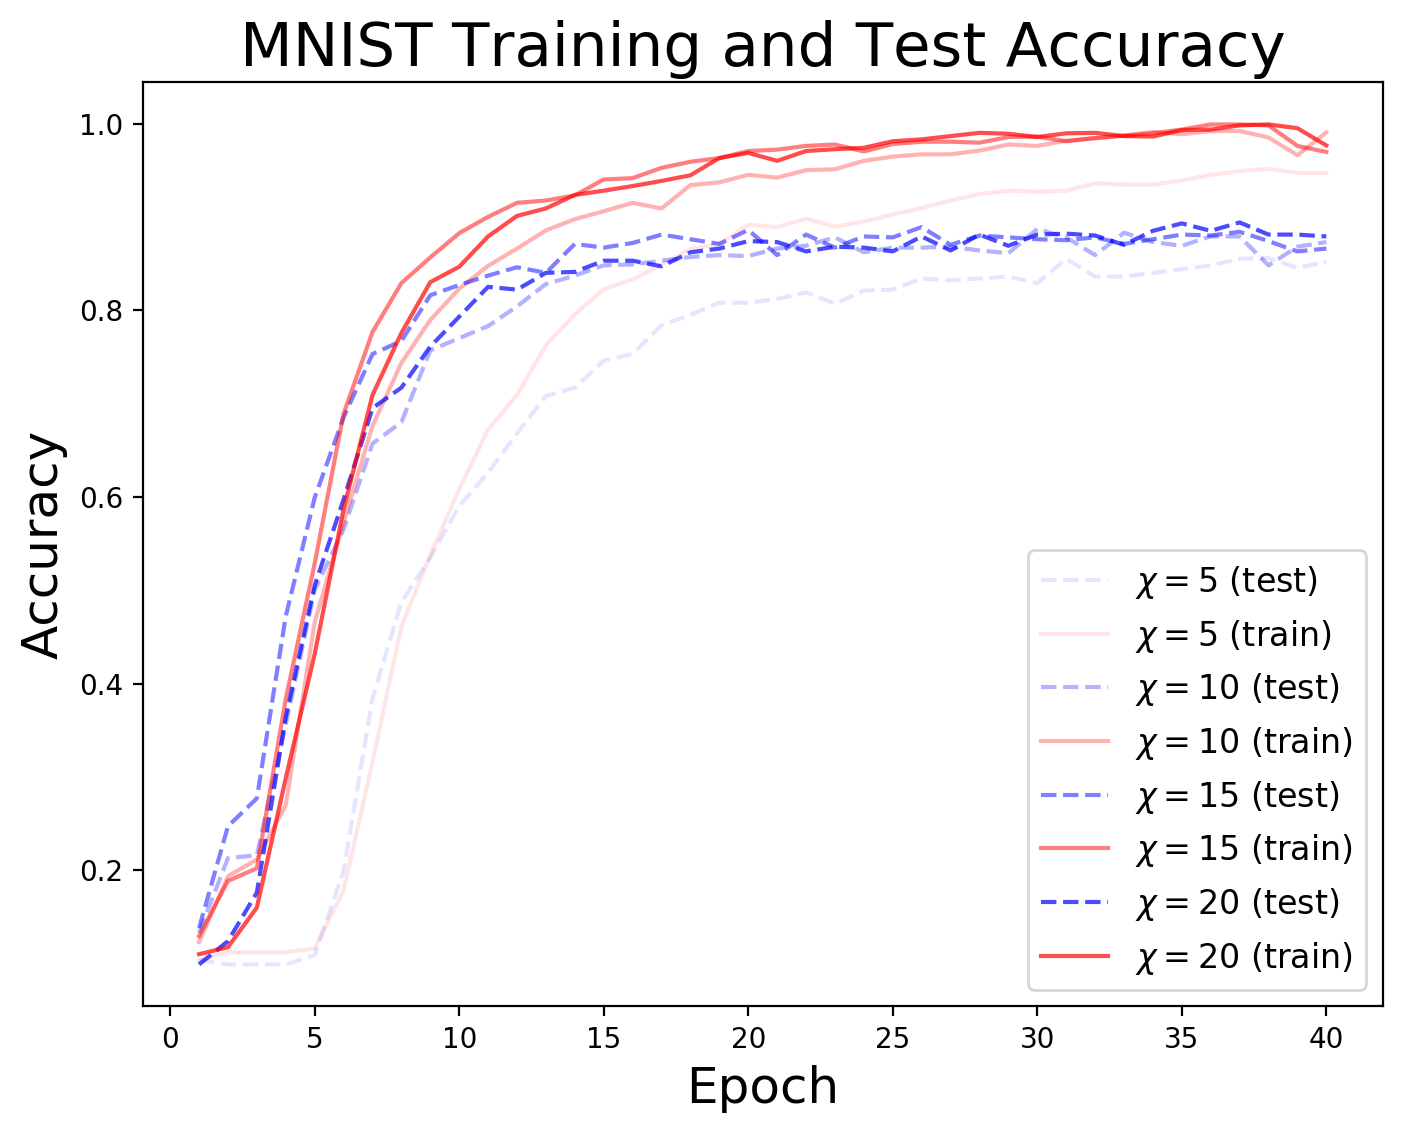
\includegraphics[width=0.62\textwidth]{MNIST_accuracies.png}
\end{frame}


\begin{frame}{Results - Regularization}
    \begin{figure}
     \begin{subfigure}
   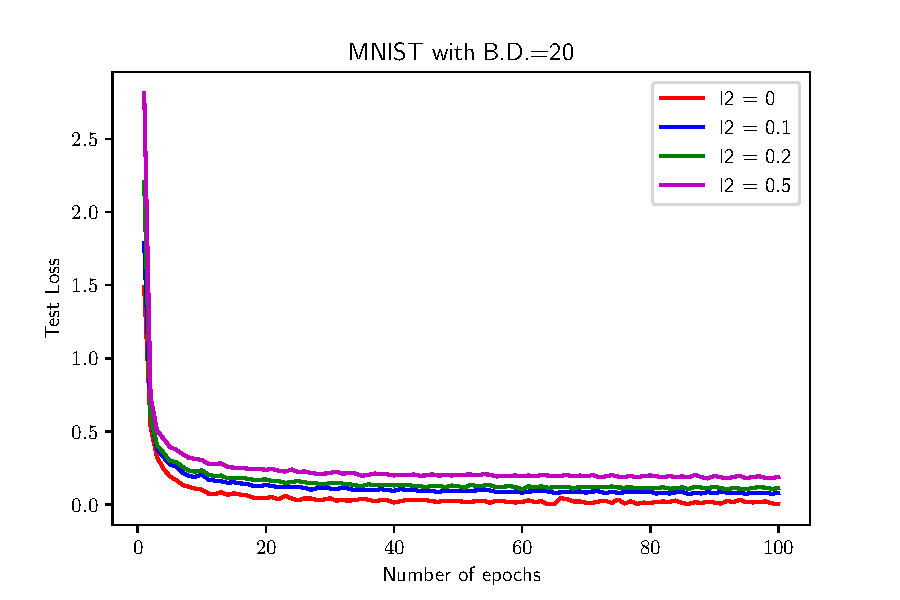
\includegraphics[width=0.45\textwidth]{mnist_l2_loss.pdf}
   \end{subfigure}
   \hfill
   \begin{subfigure}
   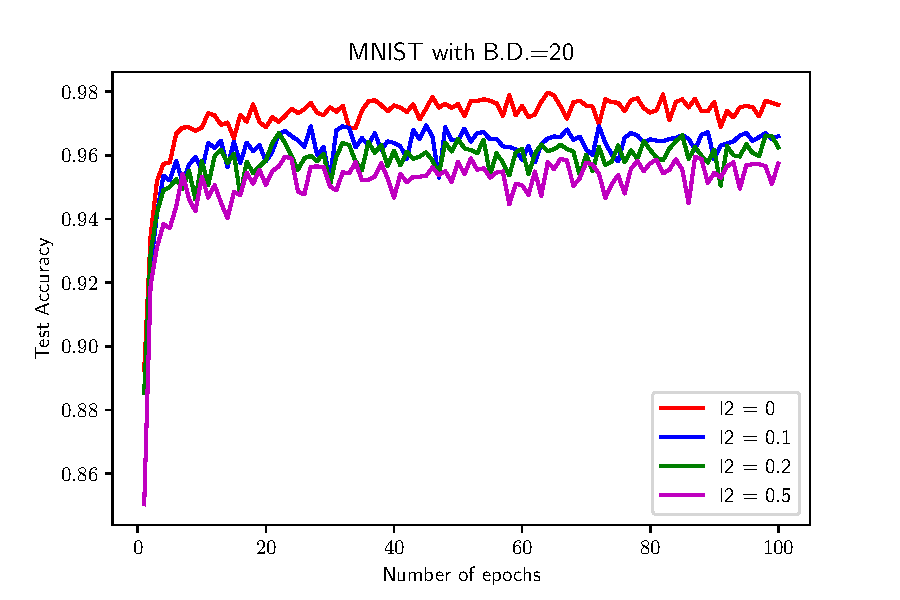
\includegraphics[width=0.45\textwidth]{mnist_l2_accuracy.pdf}
    \end{subfigure}
         \begin{subfigure}
   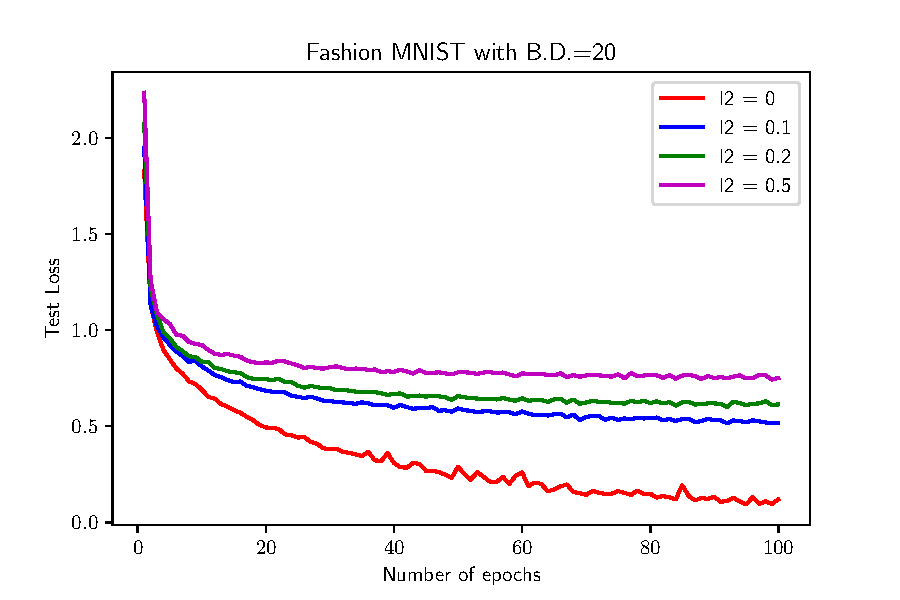
\includegraphics[width=0.45\textwidth]{fmnist_l2_loss.pdf}
   \end{subfigure}
   \hfill
   \begin{subfigure}
   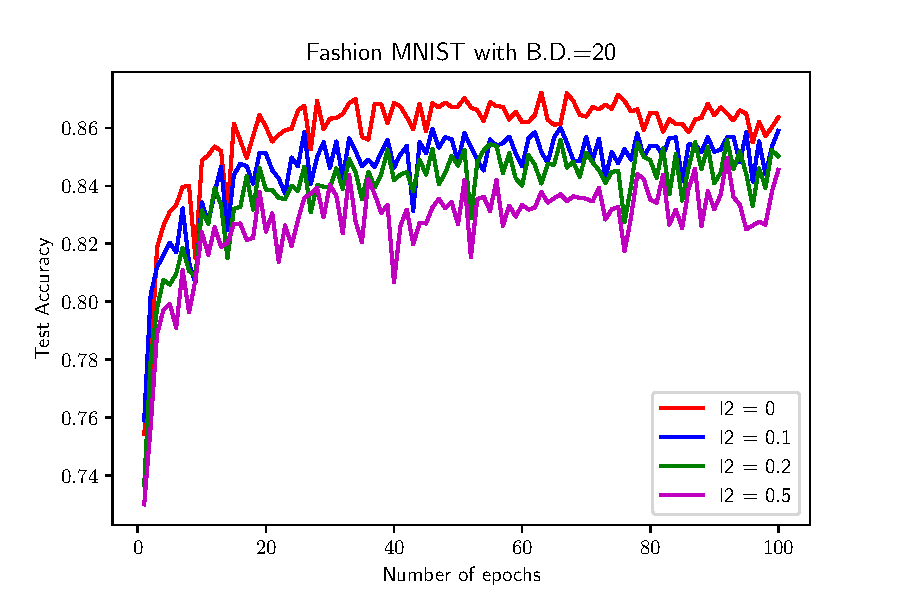
\includegraphics[width=0.45\textwidth]{fmnist_l2_accuracy.pdf}
    \end{subfigure}
    
    \end{figure}
\end{frame}



\begin{frame}{Results - Different Datasets}
    \begin{itemize}
        \item We test different datasets: MNIST, Fashion-MNIST and CIFAR10
    \end{itemize}
    \begin{figure}
      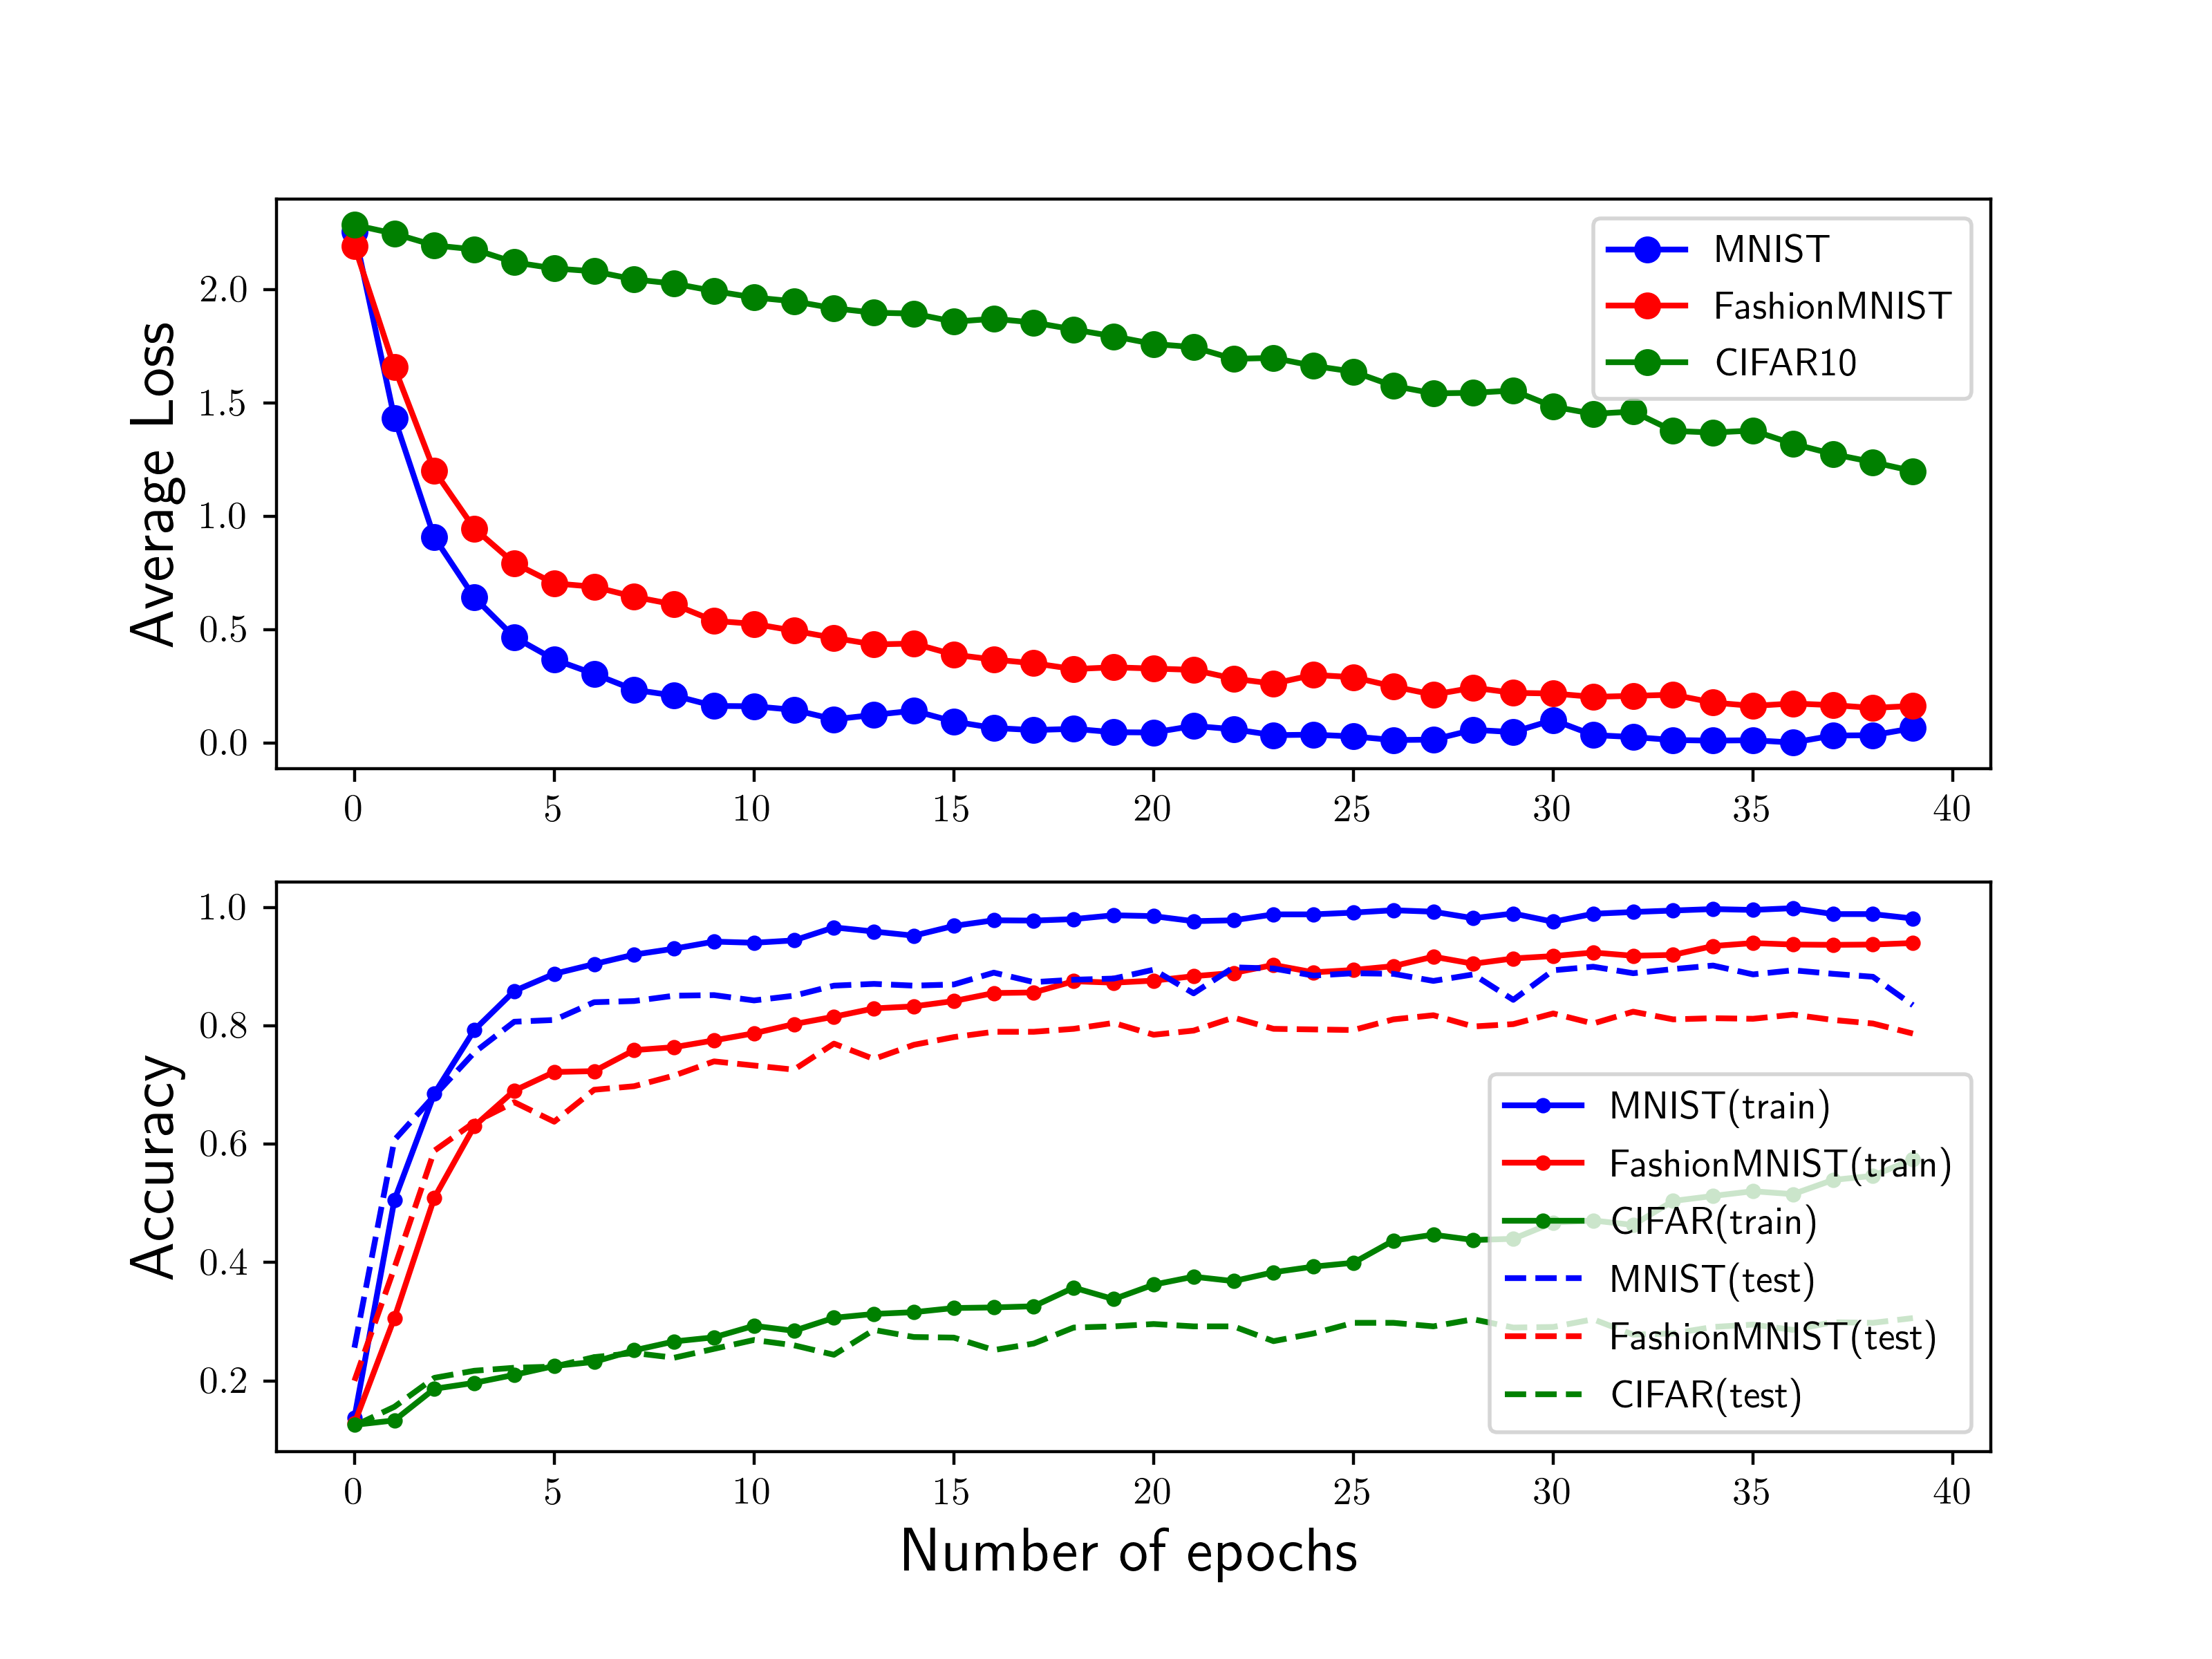
\includegraphics[width=.9\textwidth]{test.png}
    \end{figure}
\end{frame}

\begin{frame}{Results - GPU}
    \begin{itemize}
        \item We also train the dataset on GPU
    \end{itemize}
    \begin{figure}
      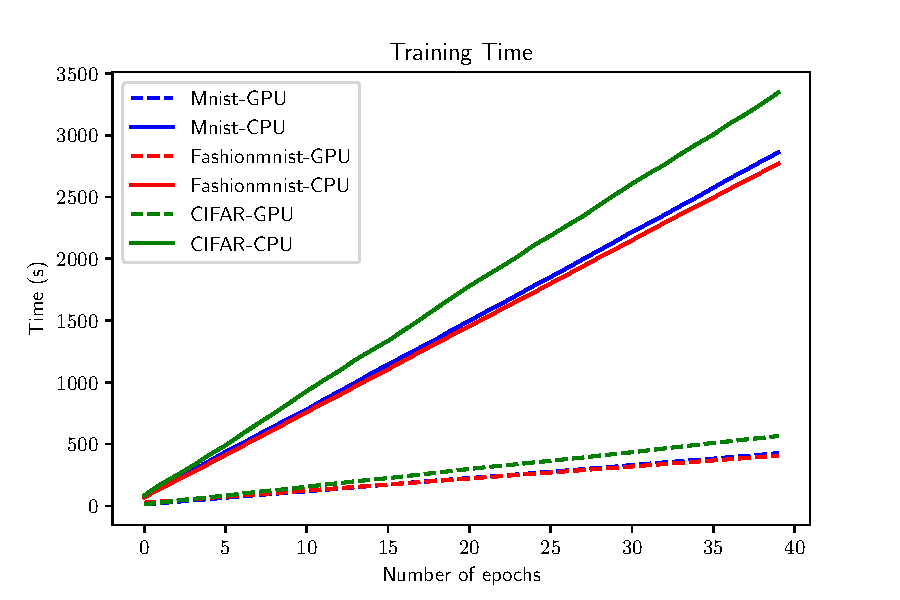
\includegraphics[width=.9\textwidth]{Running_time.pdf}
    \end{figure}
\end{frame}

\begin{frame}{Discussion and Conclusions}
    \begin{itemize}
        \item We used MPS to perform classification
        \item Large bond dimension led to better performance 
        \item Optimum test accuracy for MNIST was 96.5\%, which is comparable to existing neural networks
        \item Running code on GPU speed up our computations
        \item Potential speedup on quantum computer
    \end{itemize}
\end{frame}
    

\begin{frame}
\frametitle{}
\small
\begin{itemize}
  \item[] [1] Bridgeman, Jacob C., and Christopher T. Chubb. ``Hand-waving and interpretive dance: an introductory course on tensor networks." Journal of Physics A: Mathematical and Theoretical 50.22 (2017): 223001
  \item[] [2] Efthymiou, Stavros, Jack Hidary, and Stefan Leichenauer. ``TensorNetwork for Machine Learning." arXiv preprint arXiv:1906.06329 (2019).
  \item[] [3] Miller, Jacob. TorchMPS, 2019, \url{https://github.com/jemisjoky/torchmps}.
  \item[] [4] Stoudenmire, Edwin, and David J. Schwab. ``Supervised learning with tensor networks." Advances in Neural Information Processing Systems. 2016.

\end{itemize}
\end{frame}

\end{document}
